% WebContactsProPlus — C4 Level 2: Containers
\documentclass[border=14pt]{standalone}
\usepackage{tikz}
\usetikzlibrary{positioning, arrows.meta, shapes.geometric, fit, calc, backgrounds}

\definecolor{c4person}{HTML}{08427B}
\definecolor{c4container}{HTML}{438DD5}
\definecolor{c4db}{HTML}{438DD5}
\definecolor{c4ext}{HTML}{999999}

\begin{document}
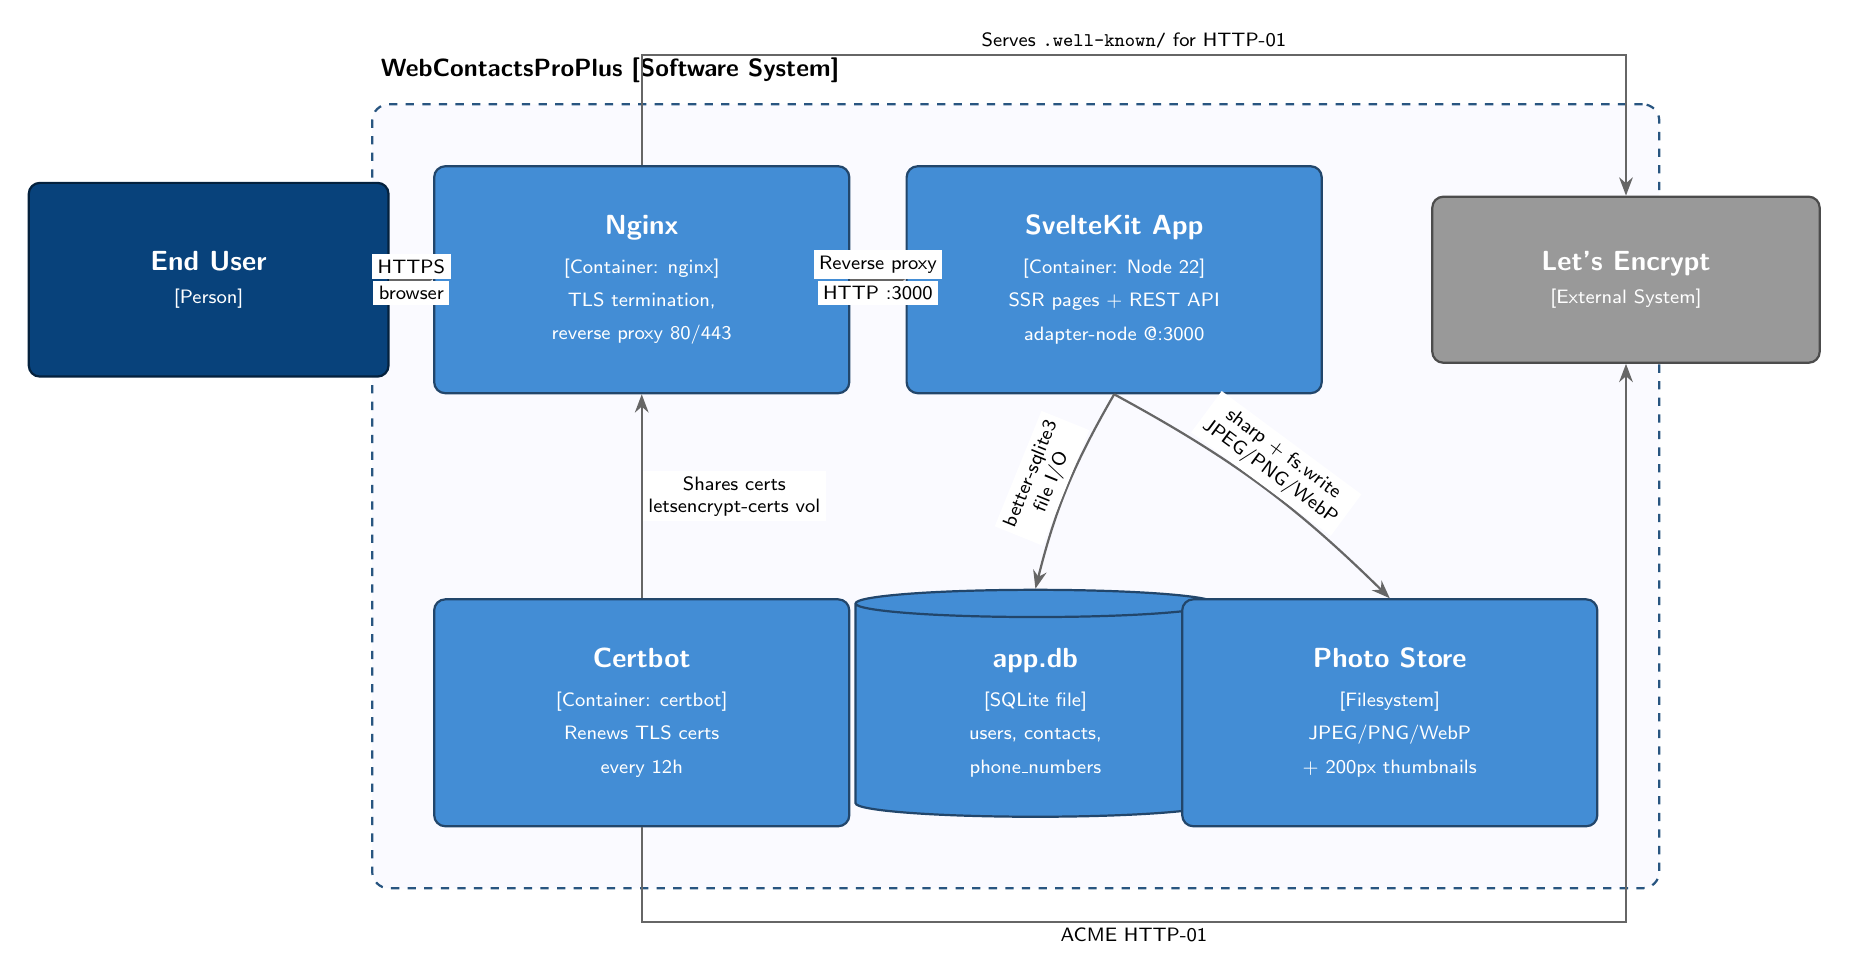
\begin{tikzpicture}[
    >=Stealth,
    font=\sffamily,
    person/.style={
        draw=c4person!50!black, fill=c4person, text=white, line width=0.8pt,
        rectangle, rounded corners=4pt,
        minimum width=130pt, minimum height=70pt, align=center,
    },
    container/.style={
        draw=c4container!50!black, fill=c4container, text=white, line width=0.8pt,
        rectangle, rounded corners=4pt,
        minimum width=150pt, minimum height=82pt, align=center,
    },
    db/.style={
        draw=c4db!50!black, fill=c4db, text=white, line width=0.8pt,
        cylinder, shape border rotate=90, aspect=0.18,
        minimum width=130pt, minimum height=82pt, align=center,
    },
    ext/.style={
        draw=c4ext!50!black, fill=c4ext, text=white, line width=0.8pt,
        rectangle, rounded corners=4pt,
        minimum width=140pt, minimum height=60pt, align=center,
    },
    boundary/.style={
        draw=c4container!60!black, dashed, line width=0.8pt, rounded corners=6pt,
        inner sep=22pt,
    },
    arrow/.style={->, line width=0.8pt, draw=black!60},
    lbl/.style={font=\sffamily\scriptsize, fill=white, inner sep=2pt, align=center},
]

% ===== Row 1 (top): End User → Nginx → SvelteKit App → Let's Encrypt =====
\node[person]    (user)  at (0, 0)    {\textbf{End User} \\ {\scriptsize [Person]}};
\node[container] (nginx) at (5.5, 0)  {
    \textbf{Nginx} \\[2pt]
    {\scriptsize [Container: nginx]} \\
    {\scriptsize TLS termination,} \\
    {\scriptsize reverse proxy 80/443}
};
\node[container] (app)   at (11.5, 0) {
    \textbf{SvelteKit App} \\[2pt]
    {\scriptsize [Container: Node 22]} \\
    {\scriptsize SSR pages + REST API} \\
    {\scriptsize adapter-node @:3000}
};
\node[ext]       (le)    at (18, 0)   {\textbf{Let's Encrypt} \\ {\scriptsize [External System]}};

% ===== Row 2 (bottom inside boundary): Certbot, app.db, Photo Store =====
\node[container] (certbot) at (5.5, -5.5)  {
    \textbf{Certbot} \\[2pt]
    {\scriptsize [Container: certbot]} \\
    {\scriptsize Renews TLS certs} \\
    {\scriptsize every 12h}
};
\node[db]        (sqlite)  at (10.5, -5.5) {
    \textbf{app.db} \\[2pt]
    {\scriptsize [SQLite file]} \\
    {\scriptsize users, contacts,} \\
    {\scriptsize phone\_numbers}
};
\node[container] (photos)  at (15, -5.5) {
    \textbf{Photo Store} \\[2pt]
    {\scriptsize [Filesystem]} \\
    {\scriptsize JPEG/PNG/WebP} \\
    {\scriptsize + 200px thumbnails}
};

% --- Boundary around the WCPP stack ---
\begin{pgfonlayer}{background}
    \node[boundary, fill=blue!2,
          fit=(nginx)(app)(sqlite)(photos)(certbot),
          label={[font=\sffamily\bfseries\small, anchor=south west, yshift=4pt]north west:WebContactsProPlus [Software System]}
    ] (sys) {};
\end{pgfonlayer}

% ===== Arrows =====
% End User → Nginx
\draw[arrow] (user) -- node[lbl, above] {HTTPS} node[lbl, below] {{\scriptsize browser}} (nginx);

% Nginx → App
\draw[arrow] (nginx) -- node[lbl, above] {Reverse proxy} node[lbl, below] {{\scriptsize HTTP :3000}} (app);

% App → Let's Encrypt is not direct — skip (nginx serves challenge, certbot makes ACME calls)

% App → SQLite (down-left)
\draw[arrow] (app.south) to[bend right=8] node[lbl, sloped, above] {better-sqlite3 \\ {\scriptsize file I/O}} (sqlite.north);

% App → Photo Store (down-right)
\draw[arrow] (app.south) to[bend left=8] node[lbl, sloped, above] {sharp + fs.write \\ {\scriptsize JPEG/PNG/WebP}} (photos.north);

% Certbot ↑ Nginx (shares cert volume)
\draw[arrow] (certbot.north) -- node[lbl, right] {Shares certs \\ {\scriptsize letsencrypt-certs vol}} (nginx.south);

% Nginx → Let's Encrypt (route up + right + down, outside boundary top)
\draw[arrow] (nginx.north) -- ++(0, 1.4) -|
    node[lbl, pos=0.25, above] {Serves \texttt{.well-known/} {\scriptsize for HTTP-01}}
    (le.north);

% Certbot → Let's Encrypt (route down + right + up, outside boundary bottom)
\draw[arrow] (certbot.south) -- ++(0, -1.2) -|
    node[lbl, pos=0.25, below] {ACME HTTP-01}
    (le.south);

\end{tikzpicture}
\end{document}
